\documentclass[11pt]{article}   %Needed for every document
\usepackage{geometry}           %Going to help get paper size right
\geometry{letterpaper}          %Normal paper
\usepackage{multicol}
\usepackage{graphicx,epsfig}    %Graphics packages and pictures
\usepackage{amssymb}            %Package for symbols

\usepackage{epstopdf}
\usepackage{color}
%\DeclareGraphicsExtensions{.pdf, .png, .jpg}
\graphicspath{ {Figures/} }
\DeclareGraphicsRule{.tif}{png}{.png}{`convert #1 `dirname #1`/`basename #1 .tif`.png}  %Need for pictures
\newcommand{\ignore}[1]{} %used to make inline comments
\definecolor{gray}{rgb}{0.5, 0.5, 0.5}
\newcommand{\gray}[1]{\colorbox{gray}{#1}}
\usepackage[utf8]{inputenc}
\usepackage[most]{tcolorbox}
\title{Hw 1}
\author{Steven Walton\\     %Note that we don't close until after address to keep in title format.
\textit{PS 232 Computational Methods}\\
\textit{Department of Physics}\\
\textit{Embry-Riddle Aeronautical University}\\
\textit{Prescott, AZ   86301}}

\tcbset{
       frame code={}
       center title,
       left=0pt,
       right=0pt,
       top=0pt,
       bottom=0pt,
       colback=gray!70,
       colframe=white,
       width=\dimexpr\textwidth\relax,
       enlarge left by=0mm,
       boxsep=5pt,
       arc=0pt,outer arc=0pt,
       }

\begin{document}

\maketitle
%This will be the objective part of the lab.

\section*{Problem 1}
For problem 1 we are asked to use the Matlab commands \gray{rand}, \gray{randn}, \gray{plot}, and \gray{polar} to generate 1000 points and the plot them.
In python we will be using the modules \gray{numpy} and \gray{matplotlib.pyplot} (here on refered to as \gray{plt}).  From these we will be using \gray{random.normal}, \gray{plt.plot},\gray{plt.show}, and \gray{plt.polar}. 
\subsection*{A}
Write a script to plot 1000 points where the x coordinates are randomly chosen from a normal distribution about 5 with a standard deviation of 1.  The y coordinate is randomly chosen to form a uniform distribution over the interval (1,5).


The following code is an example of a solution to the problem.

\begin{tcolorbox} 
   
   \noindent
      $\#$ Much of this code will be similar to MatLab since numpy is similar to MatLab\\
      \\
      from numpy import random as ran $\#$ random module will be called with ran\\
      import matplotlib.pyplot as plt $\#$ plot will be called with plti\\
      mu = 5                     $\#$ mu value for normal distribution\\
      sigma = 1                  $\#$ standard deviation\\
      N=1000                     $\#$ number of coordinates we are creating\\
      x = ran.normal(mu,sigma,N) $\#$ random numbers created with normal distribution\\ 
      y=1+4*ran.random(N)        $\#$ random numbers created between 1 and 5\\
      \\
      $\#$ Plot is almost exactly the same as MatLab's version of plot\\
      f = plt.plot(x,y,'.')      $\#$ plot the x and y coordinates with . as a marker\\
      plt.show(f)                $\#$ show the plot that is generated from above\\
   
\end{tcolorbox}

This results in the following image.\\
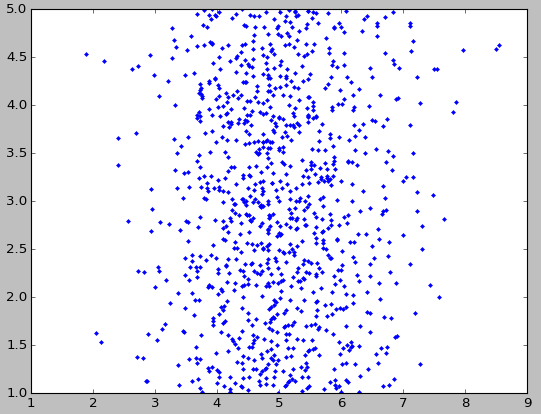
\includegraphics[scale=0.75]{Hw1Fig1.png}


\subsection*{B}
This time we will use radial coordinated with a normal distribution about 0 with width 1 and the angular coordinate theta is randomly chosen from a uniform distribution over the interval $(0,2\pi)$
\\
The code should look something like this.

\begin{tcolorbox}
   
      $\#\#$ Part 2\\
      $\#$ We are asked to plot random points in polar coordinates\\ 
      from math import pi        $\#$ We need pi for our next plot\\
      theta = 2 * pi * ran.random(N)   $\#$ randomly generated theta value, between 0 and 2pi\\
      r = ran.random(N)          $\#$ random number generated between 0 and 1\\
      p = plt.polar(theta,r,'r.')$\#$ polar plot in red\\
      plt.show(p)                $\#$ shows the plot
   
\end{tcolorbox}

This results in a figure like the following.\\
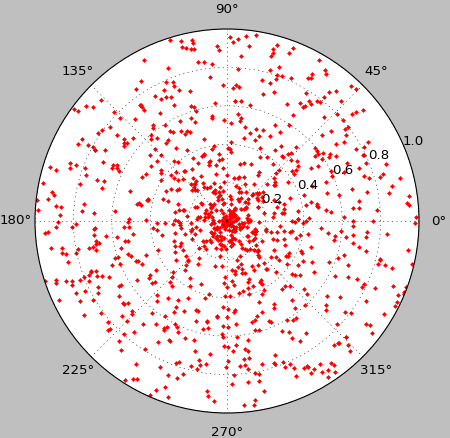
\includegraphics[scale=0.75]{Hw1Fig2}

\section*{Problem 2}
See solutions by Dr Gretarsson.
\section*{Problem 3}
We are given the equations
\[
   x=(a+b)\cos{\phi}-h\cos{\left(\frac{a+b}{b}\phi\right)}
\]
\[
   y=(a+b)\sin{\phi}-h\sin{\left(\frac{a+b}{b}\phi\right)}
\]
We are asked to set $a=2$, $b=h=1$ and run $\phi$ from $0$ to $2\pi$. We use the following code to solve the problem.

\begin{tcolorbox}
   $\#$$\#$ Problem 3 $\#$$\#$\\
   $\#$ Now we are asked to plot a parametric curve.  The equation is given for x\\
   $\#$ and y as below.  Variables are chosen for consistency and easy understanding\\
   from numpy import arange   $\#$ arange creates a list from the first to the second with specified step sizes\\
   from math import cos       $\#$ import cosine function\\
   from math import sin       $\#$ import sine function\\
   $\#$ Given variables\\
   a = 2                      \\
   b = 1\\
   h = 1\\
   step = .01\\
   $\#$ We must create empty arrays that will be updated by loop\\
   x3 = [ ]\\
   y3 = [ ]\\
   $\#$ We need to create an array in step sizes.  Step can be changed for accuracy \\
   phi = arange(0, 2*pi,step)\\
\\
   $\#$ We must use loops to append the arrays.  We will use a for loop and keep\\
   $\#$ it in the range of phi, so that when step size changes the code does not\\
   $\#$ break.\\
   i = 0    $\#$ initialize i to be zero, regardless of previously stored value\\
   for i in range(0, len(phi)):  \\
      x3.append((a + b) * cos(phi[i]) - h * cos(((a + b)/b) * phi[i]))\\
\\
   i = 0    $\#$ reinitialization of i\\
   for i in range(0, len(phi)):\\
      y3.append((a + b) * sin(phi[i]) - h * sin(((a + b)/b) * phi[i]))\\
\\
   q = plt.plot(x3,y3,'g.')   $\#$ plot the function\\
   plt.show(q)                $\#$ show the function
\end{tcolorbox}

We should get a picture like the following.
\\
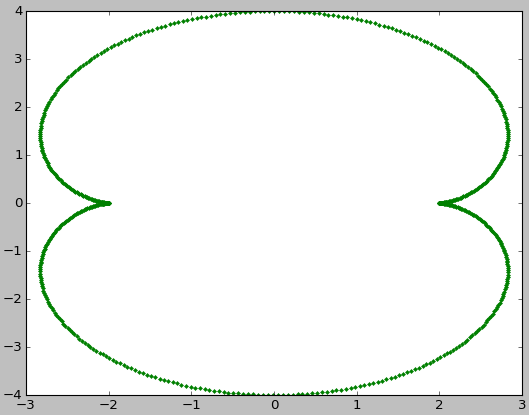
\includegraphics[scale=0.75]{Hw1Fig3.png}
\\
We are asked to plot more curves, changing a,b, and h.  This is left for the student.  The pictures will be the same as those in the MatLab solutions.

\end{document}
